
\documentclass[12pt, a4paper]{report}
\usepackage{graphicx}
\usepackage{amsmath}
\usepackage{float}
\renewcommand{\baselinestretch}{1.2} 
\usepackage{ragged2e}
\usepackage{fancyvrb}

\title{\textbf{EE2703 : Applied Programming Lab \\ Assignment 3 \\ Fitting Data to Models}} % Title
\author{Arun Krishna A M S \\ EE19B001} % Author name

\date{\today} % Date for the report

\begin{document}		
		
\maketitle % Insert the title, author and date
\justifying
\section*{Aim}
This assignment mainly focuses on
\begin{itemize}
  	\item Reading "fitting.dat" file and parse data from it
  	\item Analyze the generated data to extract information
  	\item Linear fitting to the data and the effects of noise on it
  	\item Plotting graphs for enhanced understanding
\end{itemize}

\section*{Introduction}
The assignment starts with generating data as a linear combination of the \textbf{Bessel function.} and the input variable by running the \texttt{generate\_data.py} file. To simulate real-life signals, a normally distributed noise with standard deviation sampled uniformly on a logarithmic scale has also been added. The data is stored in the \texttt{fitting.dat} file.

\begin{verbatim}
data = np.loadtxt("fitting.dat",dtype=float);	
time = np.array(data[:,0]);
data = np.array(data[:,1:]);
\end{verbatim} 
The \texttt{fitting.dat} file contains 10 columns. The first column is time, and the other 9 columns contain function:

 \begin{equation*}
 f(t) = 1.05J_2(t) - 0.105t + n(t)
 \end{equation*}
where $J_2(t)$ is the bessel function and \\
$n(t)$ is the normally distributed noise given by \\

 \begin{equation*}
\mathrm{P}(n(t)|\sigma)=\frac{1}{\sigma\sqrt{2\pi}}\text{exp}\left(-\frac{n(t)^{2}}{2\sigma^{2}}\right)
\end{equation*}
\\
where $\sigma$ is generated using \texttt{sigma=logspace(-1,-3,9)} 
\begin{center}
	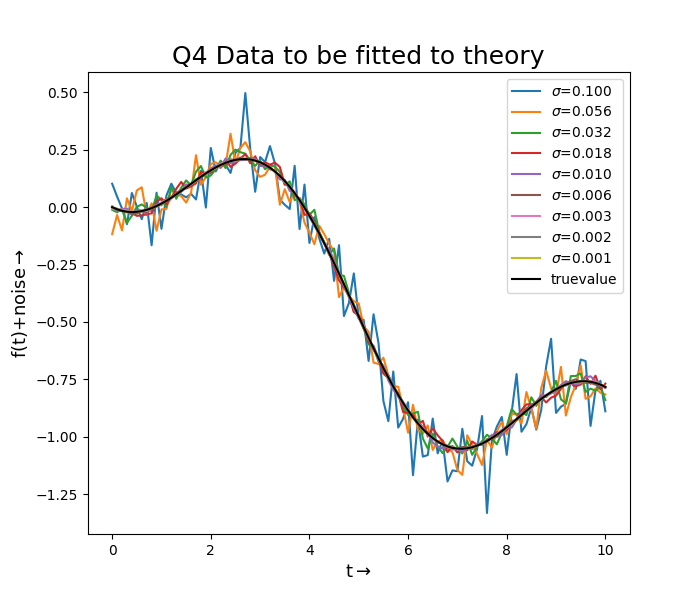
\includegraphics[scale=0.80]{Figure_0} 
	\caption{\\Plot of all data columns}
	\label{fig:rawdata}
\end{center}


\section*{Errorbar Plot}

Since the general shape of the given function is known beforehand, it is quite easy to fit the data to a model. 
\begin{equation*}
 g(t;A,B) = AJ_2(t) + Bt
\end{equation*}
where $A$ and $B$ are the parameters that needs to be figured. In this assignment we take values of the parameters as $A = 1.05$ and $B = -0.105$.
\\

Errorbar plot is an easy way of visualizing the noises present in the measurement. The first column of the data is plotted with errorbars. For readability, every $5^{th}$ item is plotted. The exact curve is also plotted to see how much the data diverges.

\begin{center}
	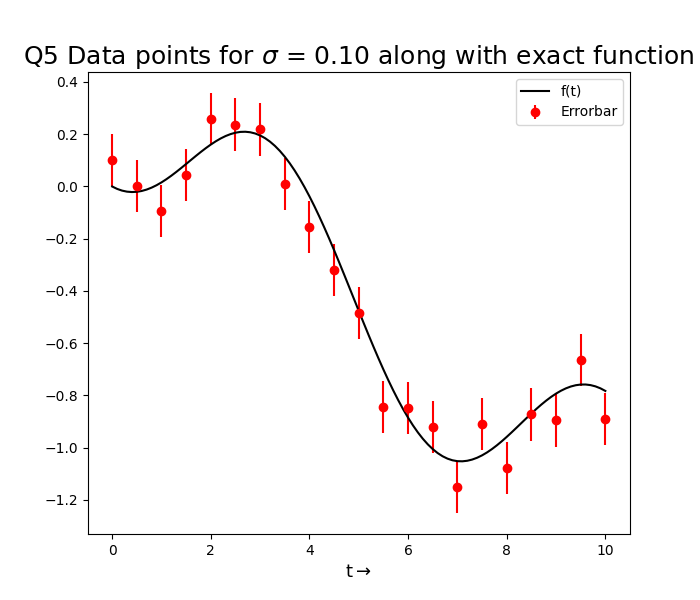
\includegraphics[scale=0.80]{Figure_1} 
	\caption{\\Errorbar Plot}
	\label{fig:rawdata}
\end{center}
\\

\section*{Matrix Generation}
Any experiment in reality, involve discreet variables. In this problem as well the variable \texttt{time} is discrete and known. Defining the matrix $M$ as 

\begin{equation*}
M=
\begin{pmatrix}
J_{2}(t_{1}) & t_{1}\\
... & ... \\
J_{2}(t_{m}) & t_{m}
\end{pmatrix}
\end{equation*}
and the vector $p$ as 
\begin{equation*}
p =
\begin{pmatrix}
A\\B
\end{pmatrix}
\end{equation*}
The vector $p$ contains the values of coefficients $A$ and $B$ and matrix $M$ which contains the Bessel function values $J_{2}(t)$ and time $t$. 

The function $g(t;A,B)$ can be written as 
\begin{equation*}
 g(t;A,B) = M\cdot p = \begin{pmatrix}
J_{2}(t_{1}) & t_{1}\\
... & ... \\
J_{2}(t_{m}) & t_{m}
\end{pmatrix}
\cdot
\begin{pmatrix}
A\\B
\end{pmatrix}
\end{equation*}

\section*{Mean Square Error Calculation}
As we traverse through $A = 0,0.1,...,2$ and $B = -0.2,-0.19,...0$, the \textbf{mean squared error} is calculated between the data $f_k$ and the assumed model using the formula

\begin{equation}\label{eq:4}
\epsilon_{ij}=\frac{1}{101}\sum_{k=0}^{101}\left(f_{k}-g(t;A,B)\right)^{2}
\end{equation} 
\\
\begin{verbatim}
A = np.linspace(0,2,21); 
B = np.linspace(-0.2,0,21); 
epsilon = np.zeros((len(A),len(B)),float);

for Ai in range(len(A)): 
    for Bi in range(len(B)): 
        error = truevalue - g(time,A[Ai],B[Bi]); 
        squareError = np.matmul(error,np.transpose(error)); 
        epsilon[Ai][Bi] = squareError/len(time); 
\end{verbatim}
The Mean squared error function values are plotted below

\begin{center}
	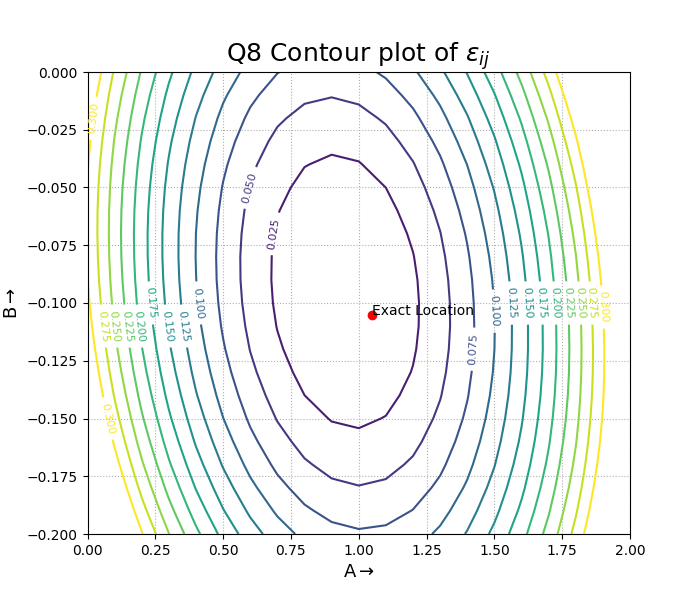
\includegraphics[scale=0.85]{Figure_2} 
	\caption{\\Mean Squared Error}
	\label{fig:rawdata}
\end{center}

The value of the paramters $A_0$ and $B_0$ corresponding to the least mean square error is the best estimate that can model the data is found using the python command:

\begin{verbatim}
Est = [np.linalg.lstsq(M,data[:,i],rcond = None)[0] for i in range(9)];
Est = np.asarray(Est);
\end{verbatim}

The \texttt{np.linalg.lstsq} function returns the least-squares solution to a linear matrix equation. Here $A_0 = 1.05$ and $B_0 = -0.105$. The error in the estimate of $A$ and $B$ for different values of $\sigma$ is plotted. It can be observed that this error is in a non-linear fashion with respect to standard deviation of noise.

\begin{center}
	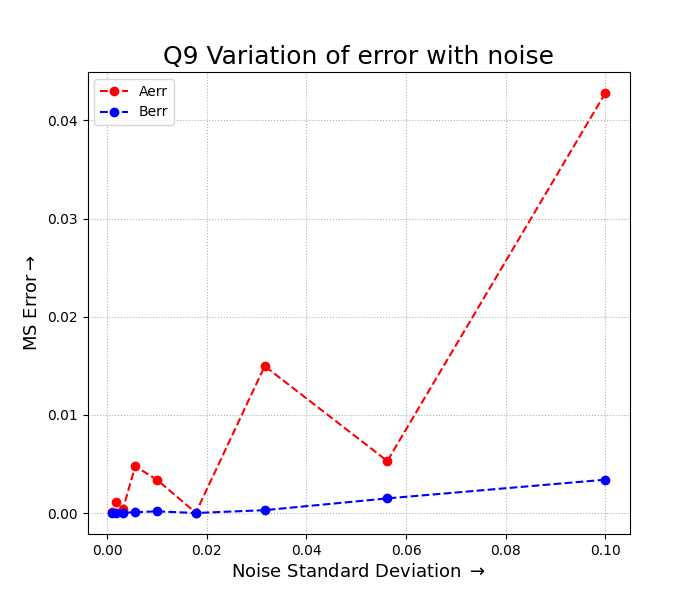
\includegraphics[scale=0.85]{Figure_3} 
	\caption{Error vs $\sigma$}
	\label{fig:rawdata}
\end{center}

On plotting on $log-log$ scale, it can be observed that the graph is approximately linear.

\begin{center}
	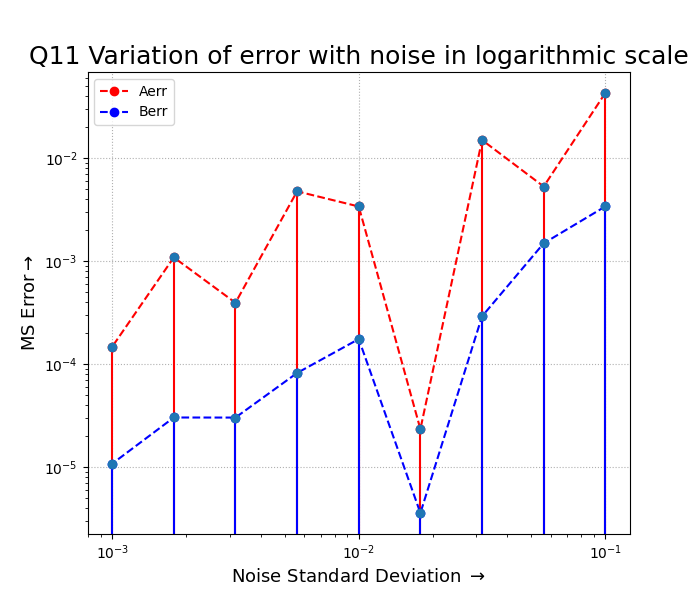
\includegraphics[scale=0.85]{Figure_4} 
	\caption{Error vs $\sigma$ in logarithmic scale}
	\label{fig:rawdata}
\end{center}

\section*{Conclusion}
A best possible fit is observed for the data obtained from the file with noises by minimizing the least mean square error. It is observed that the mean square error is directly proportional to the 
$\sigma$ of the noise in the log scale
\end{document}



 
